
\section{Additional Results} \label{AppendixA}

\subsection{Logistic regression for assistance applications}

Below we report logistic regression results for the applicant status, that is whether a county applied for federal disaster assistance based on the Public Assistance Applicants Program Deliveries data. More specifically, the applicant variable is $1$ if the county experienced a disaster and applied for dederal assistance, that is itappears in the Public Assistance Applicants Program Deliveries database, and $0$ otherwise. This is regressed on a few covariates, including the share of democratic votes in the 2016 election. All independent variables are as of 2016.


\begin{table}[htbp]
   \centering
   \caption{\label{ResultsLogit} Determinants of Assistance Application}
   \begin{tabular}{lc}
      \tabularnewline\midrule\midrule
      Dependent Variable:        & Applicant\\
      Model:                     & (1)\\
      \midrule \emph{Variables} &  \\
      (Intercept)                & -3.622\\
                                 & (3.723)\\
      Share of democratic voters & -0.8362$^{**}$\\
                                 & (0.3469)\\
      Median Income (logs)       & 0.2939\\
                                 & (0.3331)\\
      Poverty Rate               & 4.033$^{**}$\\
                                 & (1.575)\\
      Share of single mothers    & 4.068$^{***}$\\
                                 & (1.144)\\
      \midrule \emph{Fit statistics} &  \\
      Observations               & 2,882\\
      Squared Correlation        & 0.02306\\
      Pseudo R$^2$               & 0.01966\\
      BIC                        & 3,724.7\\
      \midrule\midrule\multicolumn{2}{l}{\emph{IID standard-errors in parentheses}}\\
      \multicolumn{2}{l}{\emph{Signif. Codes: ***: 0.01, **: 0.05, *: 0.1}}\\
   \end{tabular}
\end{table}





\section{Pre-Treatment Trends} \label{PreTrends}

Here we show plots of aggregated pre-treatment trends to justify the parallel trends assumption. Mean test scores are aggregated by cohort (year of first treatment) and relative time to treatment, and never treated units act as the control group. We only display these plots for overall test scores for both datasets, but not for subgroups. However, the plots for the subgroups look very similar.

\begin{figure}[!h]
	\centering
	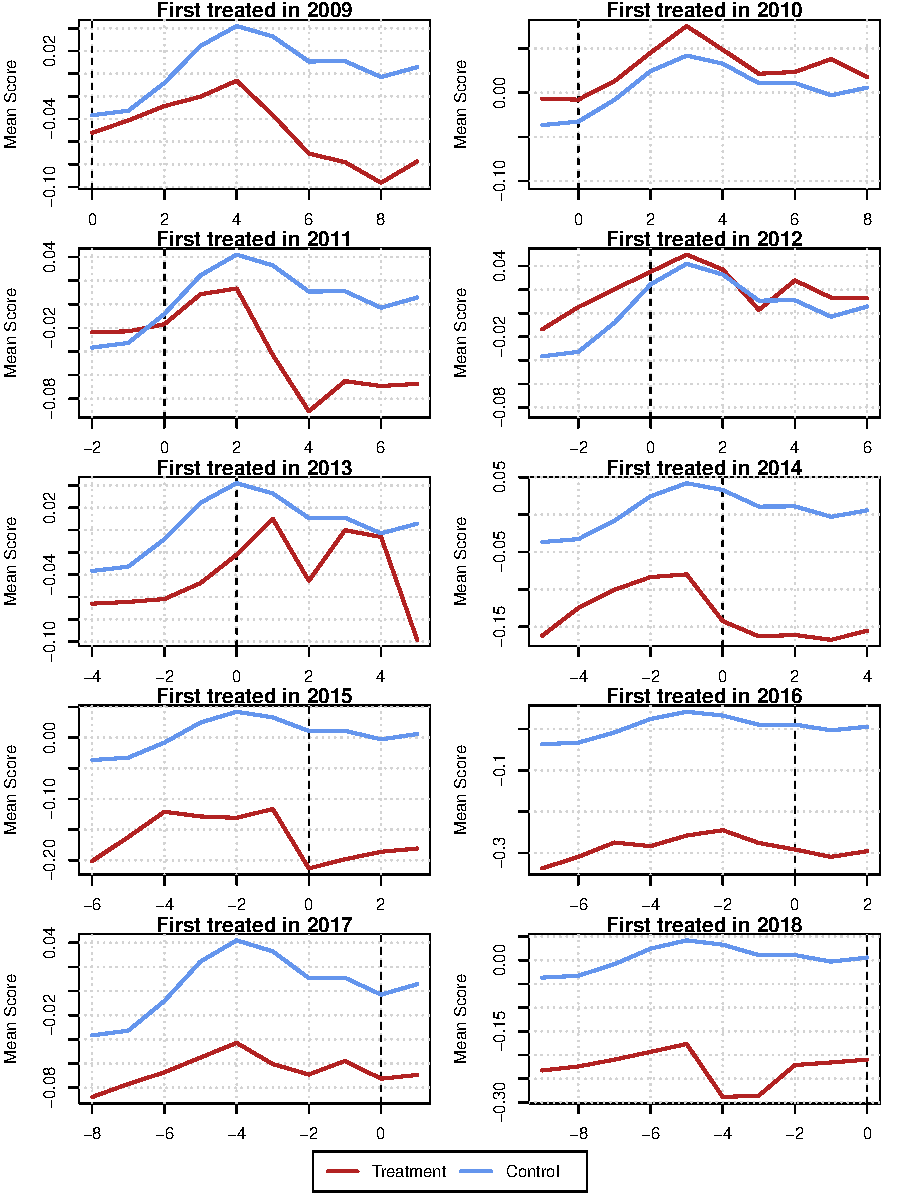
\includegraphics[scale=1]{"../Code & Data/ParTrendsPlotMathematicsFEMA.pdf"}
	\caption{Aggregated mean scores in mathematics based on FEMA data in relative time to treatment}
	\label{PreTrendsMath}
\end{figure}

\begin{figure}[!h]
	\centering
	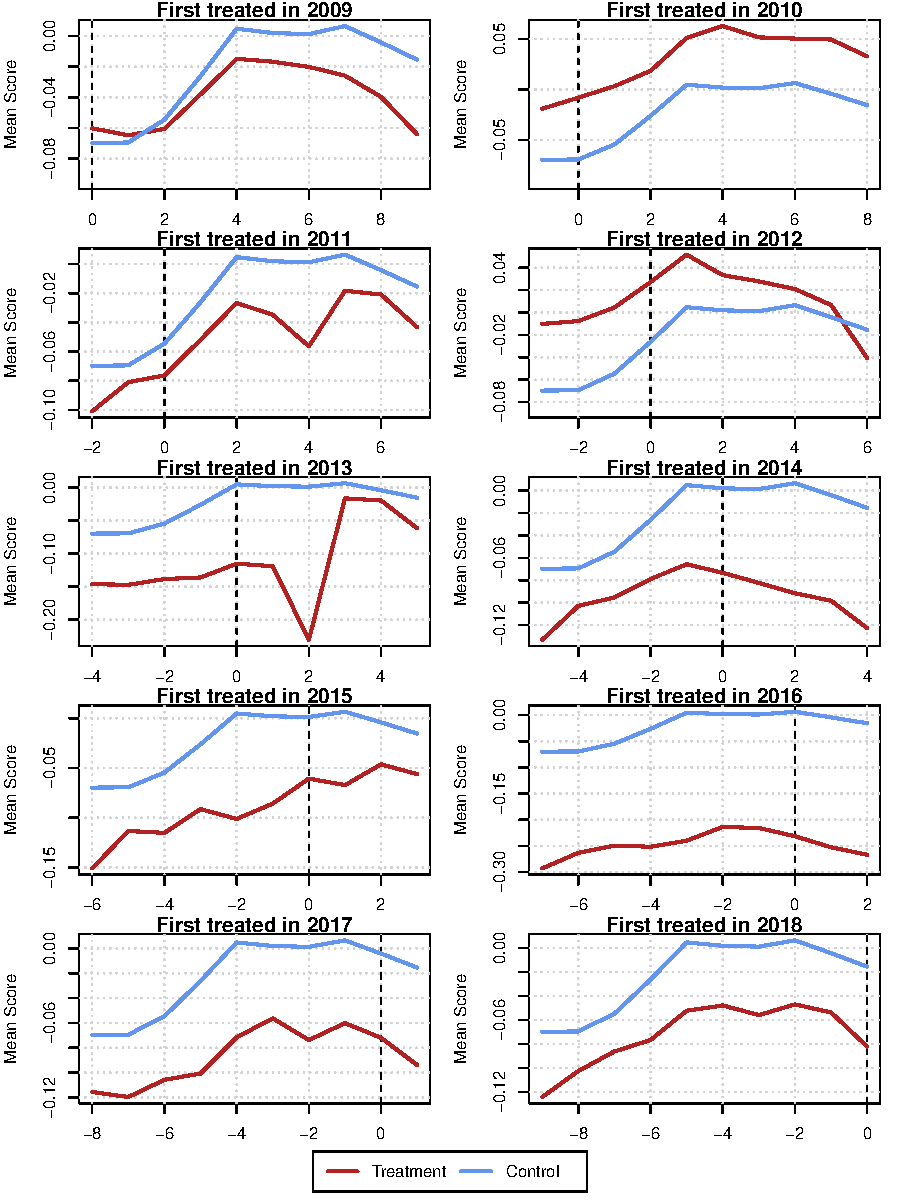
\includegraphics[scale=1]{"../Code & Data/ParTrendsPlotRLAFEMA.pdf"}
	\caption{Aggregated mean scores in RLA based on FEMA data in relative time to treatment}
	\label{PreTrendsRLA}
\end{figure}

\begin{figure}[!h]
	\centering
	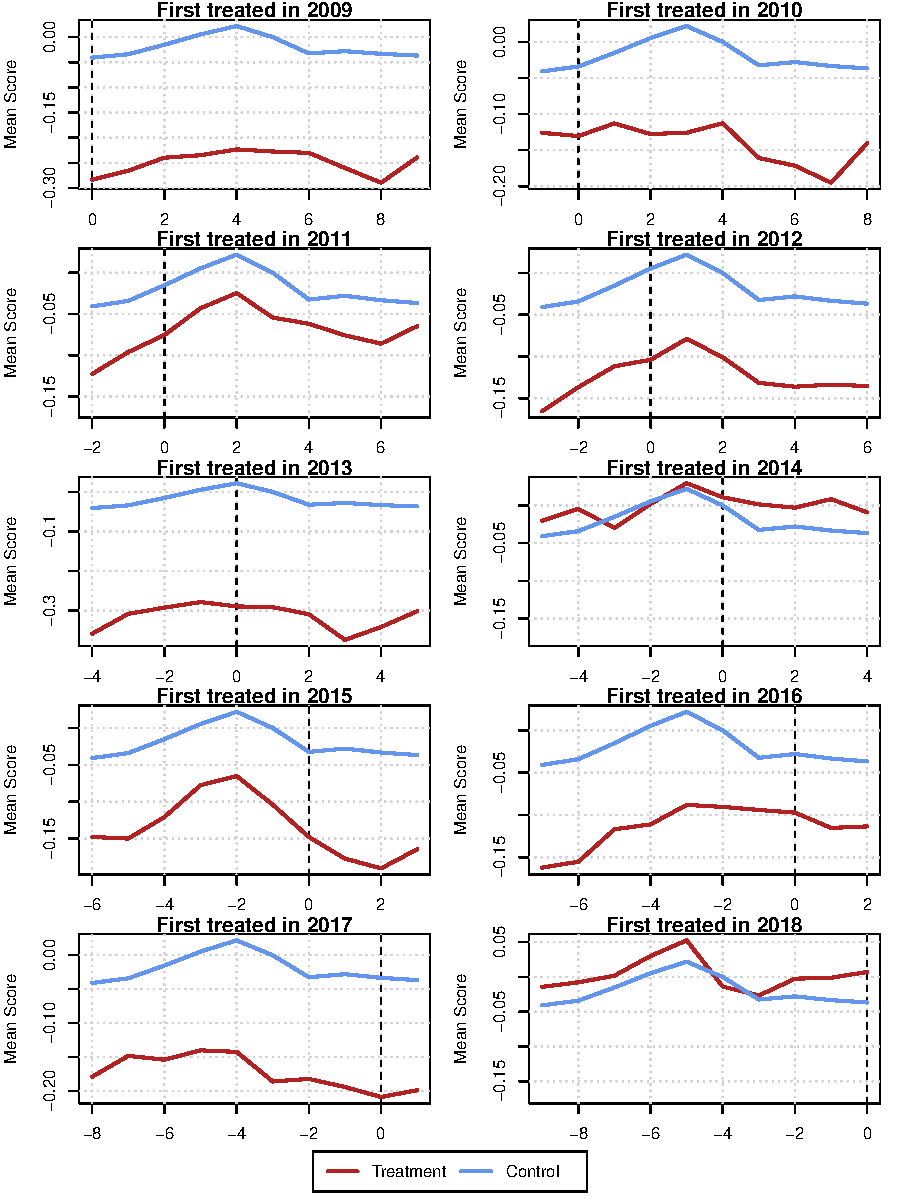
\includegraphics[scale=1]{"../Code & Data/ParTrendsPlotMathematicsStorm.pdf"}
	\caption{Aggregated mean scores in mathematics based on NWS storm data in relative time to treatment}
	\label{PreTrendsMathStorm}
\end{figure}

\begin{figure}[!h]
	\centering
	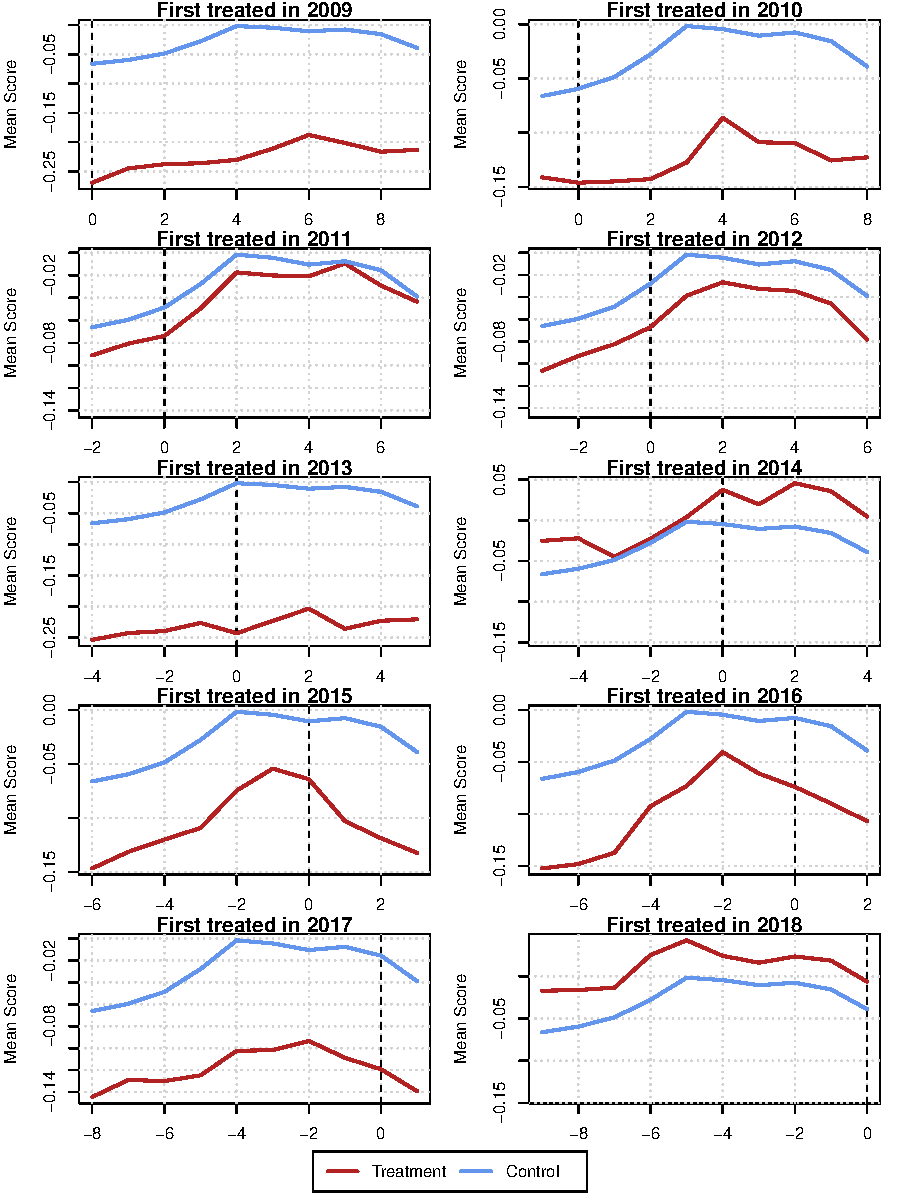
\includegraphics[scale=1]{"../Code & Data/ParTrendsPlotRLAStorm.pdf"}
	\caption{Aggregated mean scores in RLA based on NWS storm data in relative time to treatment}
	\label{PreTrendsRLAStorm}
\end{figure}

\newpage

\section{Power Analysis} \label{PowerAna}

A power analysis can be used to check how much we can trust the non-significant results. High Power implies a low type 2 error probability, that is it is unlikely to not reject the null hypothesis whent it actually should be rejected. Based on the asymptotic distribution of our estimators,
\begin{align*}
	\sqrt{N} (\widehat{\beta}_{g} - \beta_{g}) \overset{d}{\to} N(0, \sigma^2)
\end{align*}
we can compute the power of the t-test. Since, the variance has to be estimated, 
\begin{align*}
	\sqrt{N} \frac{\widehat{\beta}_{g} - \beta_{g}}{\widehat{\sigma}} \overset{a}{\sim} t(n-k),
\end{align*}
where $k$ is the number of parameters in the model. The t-test rejects $H_0: \beta_g = 0$, with probability
\begin{align*}
	\Prob \left( \lvert \sqrt{N} \frac{\widehat{\beta}_{g} - 0}{\widehat{\sigma}} \rvert \geq t_{1-\alpha/2}  \right) &= \Prob \left(  \sqrt{N} \frac{\widehat{\beta}_{g}}{\widehat{\sigma}}  \leq -t_{1-\alpha/2}  \right) + \Prob \left( \sqrt{N} \frac{\widehat{\beta}_{g}}{\widehat{\sigma}} \geq t_{1-\alpha/2}  \right) \\
	&= \Prob \left(  \sqrt{N} \frac{\widehat{\beta}_{g} - \beta_g}{\widehat{\sigma}}  \leq -t_{1-\alpha/2} - \frac{\sqrt{N}}{\widehat{\sigma}} \beta_{g}  \right) + \Prob \left( \sqrt{N} \frac{\widehat{\beta}_{g} - \beta_g}{\widehat{\sigma}} \geq t_{1-\alpha/2}  - \frac{\sqrt{N}}{\widehat{\sigma}} \beta_{g} \right) \\
	&= T\left( -t_{1-\alpha/2} - \frac{\sqrt{N}}{\widehat{\sigma}} \beta_{g} \right) + 1 - T \left(  t_{1-\alpha/2}  - \frac{\sqrt{N}}{\widehat{\sigma}} \beta_{g} \right)
\end{align*}
where $T$ is the cumulative distribution function of a t-distribution with $n-k$ degrees of freedom. Thus, for all $\beta_g \neq 0$ this expression is the power of the t-test. Using this expression, we can have a look at the power based on our data.

Figure \ref{Power} shows the power on the relative treatment indicators after treatment as a function of the true parameter value for overall mean scores based on the FEMA declarations. Power is decreasing in the temporal distance to treatment, which is not surprising since the variance increases in the temporal distance as already mentioned above. Also, power for mathematics scores tends to be lower overall than power for RLA scores. 


\begin{figure}[!h]
	\centering
	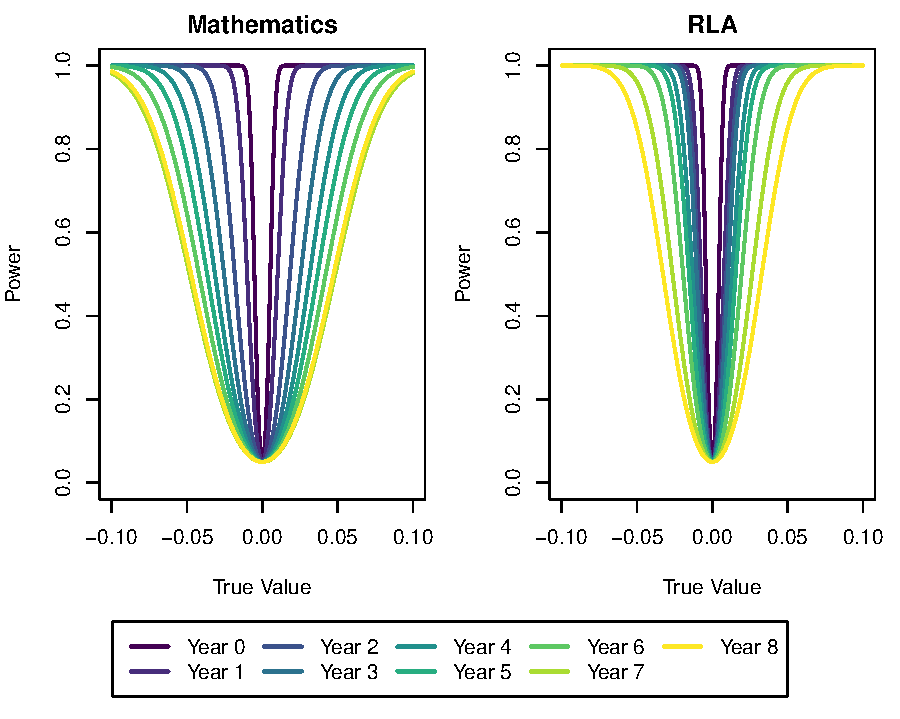
\includegraphics[scale=1]{"../Code & Data/PowerAnalysis.pdf"}
	\caption{Power of the t-test as a function of the true parameter value}
	\label{Power}
\end{figure}




